\section{Method}

We present a three-stage framework for individual-level vaccine allocation on contact networks:
(1) macro-level expert trajectory generation via ODE simulation,
(2) conditional diffusion model learning for strategy priors,
and (3) prior-guided reinforcement learning for micro-level optimization.
This section details each component.

% ============================================
\subsection{Individual-level Epidemic Dynamics on Contact Networks}
\label{sec:ctmp}

We model epidemic spread as a continuous-time Markov process (CTMP) on a contact network
$\mathcal{G} = (V, E)$, where nodes represent individuals and edges represent potential
transmission pathways.

\subsubsection{Contact Network Construction}

The population of size $N$ is partitioned into three heterogeneous groups:
\begin{itemize}
    \item \textbf{Baseline group} ($g=0$): $f_0 \approx 67.2\%$ of population
    \item \textbf{High-risk group} ($g=1$): $f_1 \approx 16.8\%$ (elderly, immunocompromised)
    \item \textbf{High-contact group} ($g=2$): $f_2 \approx 15.0\%$ (essential workers, youth)
\end{itemize}

Edge probabilities between groups are governed by a contact matrix $\mathbf{C} \in \mathbb{R}^{3 \times 3}$:
\begin{equation}
\mathbf{C} = \begin{bmatrix}
0.165 & 0.1 & 0.175 \\
0.1 & 0.0 & 0.002 \\
0.175 & 0.002 & 0.132
\end{bmatrix}
\end{equation}
where $C_{gh}$ represents the relative contact rate between groups $g$ and $h$.
This matrix reflects empirical observations that high-risk individuals (e.g., elderly)
have limited contact with high-contact groups, while high-contact individuals interact
frequently within their group and with the baseline population.

\subsubsection{State Space and Transitions}

Each individual $i \in V$ occupies one of six disease states at time $t$:
\begin{equation}
s_i(t) \in \{\text{S}, \text{E}, \text{I}, \text{R}, \text{V}, \text{D}\}
\end{equation}
where \textbf{S} = Susceptible, \textbf{E} = Exposed (latent), \textbf{I} = Infected (infectious),
\textbf{R} = Recovered, \textbf{V} = Vaccinated, \textbf{D} = Dead.

The state transition diagram is shown in Figure~\ref{fig:state_diagram}. Key features include:

\begin{itemize}
    \item \textbf{Network-dependent infection}: The force of infection for individual $i$
    depends on the states of its graph neighbors $\mathcal{N}(i)$:
    \begin{equation}
    \lambda_i(t) = \beta \cdot \frac{|\{j \in \mathcal{N}(i) : s_j(t) = \text{I}\}|}{|\mathcal{N}(i)|}
    \end{equation}
    This captures the fact that individuals with more infected neighbors face higher risk.

    \item \textbf{Vaccine-induced immunity}: Vaccinated individuals have reduced susceptibility
    $(1-\varepsilon)\lambda_i(t)$, where $\varepsilon = 0.8$ is the vaccine efficacy.

    \item \textbf{Group-dependent mortality}: Death probability $\mu_g$ varies by group,
    with $\mu_1 = 0.1$ for high-risk vs. $\mu_0 = \mu_2 = 0.01$ for others.
\end{itemize}

\begin{figure}[t]
\centering
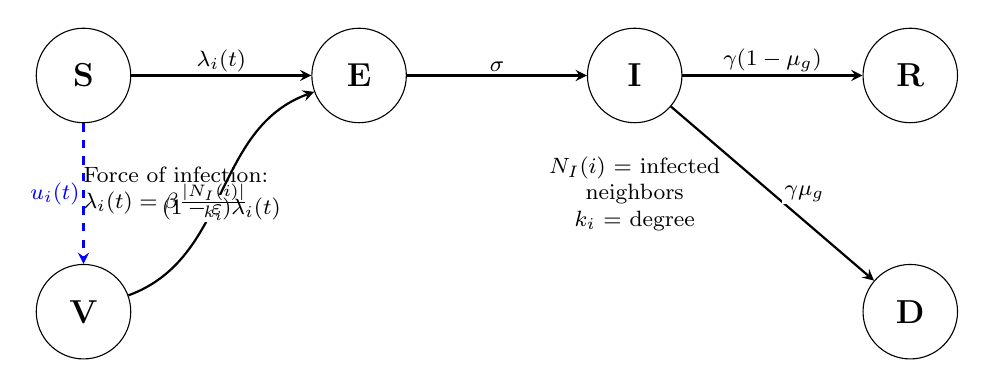
\begin{tikzpicture}[
    state/.style={circle, draw, minimum size=1.2cm, font=\bfseries\large},
    arrow/.style={->, >=stealth, thick},
    control/.style={->, >=stealth, thick, blue, dashed},
    label/.style={font=\footnotesize, midway, fill=white, inner sep=1pt}
]
    % Nodes positioned for clarity
    \node[state] (S) at (0,0) {S};
    \node[state] (E) at (3.5,0) {E};
    \node[state] (I) at (7,0) {I};
    \node[state] (R) at (10.5,0) {R};
    \node[state] (V) at (0,-3) {V};
    \node[state] (D) at (10.5,-3) {D};

    % Main disease progression
    \draw[arrow] (S) -- node[label, above] {$\lambda_i(t)$} (E);
    \draw[arrow] (E) -- node[label, above] {$\sigma$} (I);
    \draw[arrow] (I) -- node[label, above] {$\gamma(1-\mu_g)$} (R);
    \draw[arrow] (I) -- node[label, right, xshift=3pt] {$\gamma\mu_g$} (D);

    % Vaccination control
    \draw[control] (S) -- node[label, left] {$u_i(t)$} (V);

    % Breakthrough infection from V
    \draw[arrow] (V) to[out=20, in=200] node[label, below] {$(1-\varepsilon)\lambda_i(t)$} (E);

    % Annotations
    \node[font=\footnotesize, align=left, text width=3.5cm] at (1.75, -1.5)
        {Force of infection:\\$\lambda_i(t) = \beta \frac{|N_I(i)|}{k_i}$};

    \node[font=\footnotesize, text width=2.5cm, align=center] at (7, -1.5)
        {$N_I(i)$ = infected\\neighbors\\$k_i$ = degree};
\end{tikzpicture}
\caption{State transition diagram for individual-level CTMP dynamics. Solid arrows represent
disease transitions; dashed blue arrow indicates vaccination control. Unlike population-level
ODE models, the infection rate $\lambda_i(t)$ depends on the individual's network neighborhood
rather than mean-field mixing.}
\label{fig:state_diagram}
\end{figure}

\subsubsection{Discrete-time Simulation}

We implement the CTMP using discrete-time approximation with step size $\Delta t = 1$ day.
At each time step, state transitions occur stochastically according to Algorithm~\ref{alg:ctmp_step}.

\begin{algorithm}[h]
\caption{CTMP Simulation (one time step)}
\label{alg:ctmp_step}
\begin{algorithmic}[1]
\STATE \textbf{Input:} Current states $\{s_i(t)\}_{i=1}^N$, graph $\mathcal{G}$, actions $\{a_i(t)\}$
\STATE \textbf{Output:} Next states $\{s_i(t+1)\}_{i=1}^N$
\STATE
\FOR{each individual $i \in V$}
    \IF{$s_i(t) = \text{S}$ and $\text{rand}() < a_i(t)$}
        \STATE $s_i(t+1) \gets \text{V}$ \hfill $\triangleright$ Vaccination
    \ELSIF{$s_i(t) \in \{\text{S}, \text{V}\}$}
        \STATE $n_I \gets |\{j \in \mathcal{N}(i) : s_j(t) = \text{I}\}|$ \hfill $\triangleright$ Count infected neighbors
        \STATE $p_{\text{infect}} \gets \beta \cdot n_I / |\mathcal{N}(i)|$
        \IF{$s_i(t) = \text{V}$}
            \STATE $p_{\text{infect}} \gets (1-\varepsilon) \cdot p_{\text{infect}}$ \hfill $\triangleright$ Vaccine protection
        \ENDIF
        \IF{$\text{rand}() < p_{\text{infect}}$}
            \STATE $s_i(t+1) \gets \text{E}$ \hfill $\triangleright$ New infection
        \ENDIF
    \ELSIF{$s_i(t) = \text{E}$ and $\text{rand}() < \sigma$}
        \STATE $s_i(t+1) \gets \text{I}$ \hfill $\triangleright$ Symptom onset
    \ELSIF{$s_i(t) = \text{I}$ and $\text{rand}() < \gamma$}
        \IF{$\text{rand}() < \mu_{g(i)}$}
            \STATE $s_i(t+1) \gets \text{D}$ \hfill $\triangleright$ Death
        \ELSE
            \STATE $s_i(t+1) \gets \text{R}$ \hfill $\triangleright$ Recovery
        \ENDIF
    \ENDIF
\ENDFOR
\end{algorithmic}
\end{algorithm}

\textbf{Parameters:} We use epidemiologically calibrated values based on COVID-19 literature:
$\beta = 0.05$ (transmission rate per contact per day),
$\sigma = 1/4$ (incubation rate, corresponding to 4-day average latent period),
$\gamma = 1/7$ (recovery rate, corresponding to 7-day average infectious period),
$\varepsilon = 0.8$ (vaccine efficacy),
and group-specific death rates $\mu_0 = \mu_2 = 0.01$, $\mu_1 = 0.1$ reflecting the
10-fold higher mortality risk in the high-risk group.

\subsubsection{Control Problem Formulation}

The vaccine allocation problem is formulated as a finite-horizon Markov Decision Process (MDP)
with the following components:

\begin{itemize}
    \item \textbf{State space} $\mathcal{S}$: The full system state $s_t = (\{s_i(t)\}_{i=1}^N, \mathcal{G}, \{g_i\}_{i=1}^N, t)$
    includes individual disease states, the contact network structure, group memberships, and time.

    \item \textbf{Action space} $\mathcal{A}$: At each time $t$, the policy outputs vaccination
    probabilities $a_t = (a_1(t), \ldots, a_N(t)) \in [0,1]^N$ subject to the supply constraint:
    \begin{equation}
    \sum_{i=1}^N a_i(t) \cdot \mathbb{I}[s_i(t) = \text{S}] \leq V_{\max}
    \label{eq:supply_constraint}
    \end{equation}
    where $V_{\max}$ is the daily vaccine supply (typically $V_{\max} = 10$ for $N=2000$).

    \item \textbf{Transition dynamics} $P(s_{t+1} | s_t, a_t)$: Governed by the stochastic
    CTMP simulation described in Algorithm~\ref{alg:ctmp_step}.

    \item \textbf{Reward function}: We seek to minimize cumulative infections and deaths:
    \begin{equation}
    r_t = -\left( |\{i : s_i(t) = \text{I}\}| + 10 \cdot |\{i : s_i(t) = \text{D}\}| \right)
    \label{eq:reward}
    \end{equation}
    The coefficient 10 assigns higher penalty to deaths, reflecting the value of life in
    public health decision-making.

    \item \textbf{Objective}: Find the optimal policy $\pi^*: \mathcal{S} \to \Delta(\mathcal{A})$
    that maximizes expected cumulative reward over horizon $T$:
    \begin{equation}
    \pi^* = \arg\max_{\pi} \mathbb{E}_{\tau \sim P_\pi} \left[ \sum_{t=0}^{T-1} r_t \right]
    \label{eq:objective}
    \end{equation}
    where $\tau = (s_0, a_0, r_0, s_1, \ldots)$ denotes a trajectory.
\end{itemize}

\paragraph{Comparison to ODE Framework.}
Unlike population-level ODE models~\citep{师兄论文} that assume homogeneous mixing within
groups via contact matrices $\mathbf{C}$, our CTMP formulation explicitly models individual
heterogeneity in contact patterns. For instance, two individuals in the high-contact group
may have degrees $k_i = 5$ and $k_j = 15$, leading to different infection risks ($\lambda_i \propto k_i$)
and vaccination priorities. This network-aware modeling enables \emph{degree-based targeting strategies}---prioritizing
high-degree ``super-spreaders''---that are fundamentally impossible in the group-level ODE framework
where all individuals within a group are treated identically.

% ============================================
\subsection{Macro-level Expert Trajectory Generation}
\label{sec:ode_expert}

\textit{[To be written: ODE simulation using ProtectorPrevent, group-level strategies (high-risk, high-contact, uniform), generating 1000 macro-level expert trajectories]}

% ============================================
\subsection{Macro-to-Micro Lifting Algorithm}
\label{sec:lifting}

\textit{[To be written: Degree-risk weighted lifting, feasibility projection, Algorithm for mapping $U_g(t) \in \mathbb{R}^3 \to a_i(t) \in [0,1]^N$]}

% ============================================
\subsection{Conditional Diffusion Model for Strategy Prior}
\label{sec:diffusion}

\textit{[To be written: DDPM formulation, Transformer architecture, conditional encoding of state features, training on lifted expert data]}

% ============================================
\subsection{Prior-Guided Reinforcement Learning}
\label{sec:rl}

\textit{[To be written: PPO algorithm, KL regularization to diffusion prior, loss function with $\beta$ annealing, training procedure]}

